\documentclass[10pt]{article}
\usepackage[letterpaper,margin=0.76in]{geometry}
\usepackage[T1]{fontenc}
\usepackage{lmodern}
\usepackage{microtype}
\usepackage{amsmath,amssymb,mathtools}
\usepackage{booktabs}
\usepackage{array}
\usepackage{graphicx}
\usepackage{xcolor}
\usepackage{titlesec}
\usepackage[font=small,labelfont=bf,skip=4pt,hypcap=false]{caption}
\usepackage[numbers,sort&compress]{natbib}
\usepackage[most]{tcolorbox}
\usepackage{enumitem}
\usepackage{hyperref}

\definecolor{ink}{HTML}{1F2933}
\definecolor{muted}{HTML}{66737F}
\definecolor{accent}{HTML}{394B59}
\definecolor{boxbg}{HTML}{F2F5F7}
\hypersetup{colorlinks=true,linkcolor=accent,urlcolor=accent,citecolor=accent}
\color{ink}

\titleformat{\section}{\large\bfseries\color{accent}}{}{0pt}{}
\titlespacing*{\section}{0pt}{0.75em}{0.25em}
\setlength{\parindent}{0pt}
\setlength{\parskip}{0.40em}
\setlength{\bibsep}{1pt}
\renewcommand{\bibfont}{\footnotesize}

% --- Conceptual Persuasions callout -------------------------------------
\newtcolorbox{cpbox}{
  enhanced, breakable,
  colback=boxbg, colframe=boxbg,
  boxrule=0pt, arc=2.5pt, outer arc=2.5pt,
  left=10pt, right=10pt, top=7pt, bottom=8pt,
  borderline west={2.4pt}{0pt}{accent},
  before skip=0.95em, after skip=0.95em,
}
\newenvironment{persuasions}
  {\begin{cpbox}\small\setlength{\parskip}{0pt}%
   {\footnotesize\bfseries\color{accent}%
    \textls[110]{CONCEPTUAL PERSUASIONS}}\par\vspace{3pt}%
   \begin{itemize}[leftmargin=1.15em,itemsep=2.5pt,topsep=0pt,parsep=0pt,
                   label=\textcolor{accent}{\scriptsize$\blacktriangleright$}]}
  {\end{itemize}\end{cpbox}}

\title{\vspace{-2.3em}\textbf{Noether Constraints and the Measure of Compatible Histories}}
\author{J. R. Landers}
\date{}

\begin{document}
\maketitle
\vspace{-1.25em}

\begin{abstract}
The accumulated-history approach to cosmology begins with a striking scale
connection: if a three-dimensional state acquires three effective distinctions
per doubling of cosmic age, then the Hubble expansion rate is $H=1/t$, and the
benchmark age of the Universe gives
$H_0=70.85\,\mathrm{km\,s^{-1}\,Mpc^{-1}}$.  The next question is more
fundamental than the numerical coincidence: what makes two histories
compatible, and what measure turns their disappearance into information?
This note develops that missing layer through a sequence of controlled tests.
A conditional survival estimator correctly removes predictable expansion and
deterministic chaos while recovering injected information rates.  A geometric
tolerance, however, does not define a unique continuum bit rate.  Conservation
then supplies physical admissibility.  Following Noether's connection between
time-translation symmetry and energy conservation, candidate transitions are
restricted to cells intersecting an energy shell, and accumulated paths are
restricted by a discrete stationary-action equation.  The raw cardinalities
exhibit universal spatial and temporal refinement terms.  Their finite
cell-count remainder converges but is not invariant under grid deformation or
canonical coordinates.  Liouville phase-volume density is different: it agrees
across those choices to better than $0.26\%$ for both harmonic and anharmonic
Hamiltonians.  The result advances the program from an arbitrary neighborhood
count to an invariant measure and isolates the remaining physical task: define
a covariant conditional history measure and its continuum time normalization.
\end{abstract}

\section*{From the Hubble scale to a measurement problem}

The preceding note, \emph{Hubble Scale from Time-Induced Complexity}, began
with a simple relational theorem.  When nonnegative distinguishing
coordinates are appended to an additive distance, fixed-radius neighborhoods
can only lose members.  If $\rho(t)$ denotes the fraction of alternative
histories still compatible with a present history, define
\begin{equation}
C(t)\equiv-\log_2\rho(t).
\label{eq:complexity}
\end{equation}
Here $t$ is cosmic time and $\log_2$ is the base-two logarithm, so $C$ is
measured in bits.  Identifying inverse compatible-history density with a
dimensionless relational volume and taking its three-dimensional linear scale
gives the proposed bridge
\begin{equation}
a_{\rm rel}(t)\propto2^{C(t)/3},
\qquad
H_{\rm rel}(t)=\frac{\ln2}{3}\dot C(t).
\label{eq:bridge}
\end{equation}
Here $a_{\rm rel}$ is the hypothesized relational scale factor,
$H_{\rm rel}\equiv\dot a_{\rm rel}/a_{\rm rel}$ is its fractional expansion
rate, an overdot means $d/dt$, and $\ln$ is the natural logarithm.  The
scale-free ansatz $C(t)=3\log_2(t/t_*)+C_*$, with arbitrary reference time
$t_*>0$ and $C_*=C(t_*)$, then gives $H(t)=1/t$ after identifying
$a_{\rm rel}$ with the physical cosmological scale factor.  From the benchmark
present age $t_0=13.80\,\mathrm{Gyr}$ and defining $H_0\equiv H(t_0)$,
\begin{equation}
H_0^{\rm age}=70.85\,\mathrm{km\,s^{-1}\,Mpc^{-1}}.
\label{eq:hubble-scale}
\end{equation}
As emphasized in the preceding note, the age is itself inferred within a
cosmological model, so this is a scale connection rather than an independent
measurement of $H_0$.  The match remains suggestive.  Its strongest reading
is not that three fixed channels describe every epoch---Dark Energy
Spectroscopic Instrument (DESI) Data Release 2 distances already exclude that
constant-power history \citep{DESI2025}---but that cosmic expansion and the
rate at which histories become distinguishable may share a natural scale.

Equation~\eqref{eq:bridge} makes the next requirement exact.  A cosmological
claim needs a $C(t)$ defined without using $H(t)$, together with a measure of
compatibility that survives changes of coordinates, resolution, and time
slicing.  Otherwise a chosen radius or discretization can set the apparent bit
rate.  This note asks whether the relational idea can be carried from a
combinatorial neighborhood into classical dynamics in a principled way.

\begin{persuasions}
\item The original clue remains $H_0t_0\simeq1$: the present expansion rate is
naturally comparable to the inverse accumulated age.
\item A clue becomes a physical model only when ``compatible history'' has an
independent operational meaning.
\item The decisive object is not merely a count.  It is a count or measure that
does not change when the same physics is described with different coordinates
or numerical resolution.
\item This shifts the problem from inventing a better cosmological fit to
identifying the correct measure on histories.
\end{persuasions}

\section*{Conditional survival of histories}

Represent history $h_i$ by states $x_i(s)$ at ordered slices
$s=0,1,\ldots$, where a slice is one step in the chosen temporal
coarse-graining.  Consider pairs $h_i,h_j$ drawn from an ensemble conditioned
to share the same resolved past.  Let $F_s$ be a predictor fixed before the
comparison that maps a state at slice $s$ to its predicted successor.  Define
the innovation---the part not predicted from the preceding resolved state---by
\begin{equation}
\epsilon_i(s+1)=x_i(s+1)-F_s[x_i(s)].
\label{eq:innovation}
\end{equation}
For a nonnegative dissimilarity $d(u,v)\geq0$ between two innovations, the
cumulative conditional distance through discrete slice $N$ is
\begin{equation}
\delta_N(i,j)=\sum_{s<N}d\!\left(\epsilon_i(s+1),\epsilon_j(s+1)\right).
\label{eq:cumulative-distance}
\end{equation}
At fixed tolerance $r\geq0$, the survival fraction and information are
\begin{equation}
\rho_N(r)=\Pr[\delta_N(i,j)\le r\mid\text{shared resolved past}],
\qquad C_N(r)=-\log_2\rho_N(r).
\label{eq:survival}
\end{equation}
where $\Pr$ is probability over the conditioned pair ensemble.  Because every
summand in Eq.~\eqref{eq:cumulative-distance} is nonnegative,
the compatible sets are nested in time.  The construction is therefore the
history analogue of the original neighborhood filtration.

Four laptop-scale controls, using fixed seed $20260824$ and ensembles of up to
two million history pairs, tested what the estimator counts.  Predictable
uniform expansion raised raw fixed-radius complexity from $1.0000$ to
$1.9546$ bits, but exact conditioning reduced it to zero.  A deterministic
chaotic standard map---an area-preserving discrete dynamical system---produced
$0.5581$ raw bits at the test radius and again zero after conditioning.
Independent binary innovations injected at exactly
one bit per update were recovered at $1.0022$ bits per update; grouping two
updates at a time returned $1.0010$ bits per primitive update.  Finally, a
deterministic hidden bit tape yielded $0.9971$ bits per update to an observer
conditioned only on the revealed macro-history, while an observer given the
complete microstate measured zero.

\begin{center}
\captionof{table}{Controlled tests of conditional history survival.  Raw
separation can be generated by known expansion or deterministic chaos;
conditional novelty removes both and recovers genuinely unresolved distinctions.}
\label{tab:controls}
\small
\begin{tabular}{>{\raggedright\arraybackslash}p{0.36\linewidth}
                >{\raggedright\arraybackslash}p{0.25\linewidth}
                >{\raggedright\arraybackslash}p{0.28\linewidth}}
\toprule
System & Unconditioned or coarse result & Correctly conditioned result\\
\midrule
Predictable uniform expansion & $1.9546$ raw bits & $0$ bits\\
Deterministic standard map & $0.5581$ raw bits & $0$ bits\\
One injected random bit/update & --- & $1.0022$ bits/update\\
Fixed hidden bit tape & $0.9971$ bits/update & $0$ with full microstate\\
\bottomrule
\end{tabular}
\end{center}

The distinction is important.  Histories can separate because an already
known flow carries them apart, because deterministic chaos amplifies an
initial difference, or because information unavailable in their shared past
is newly revealed.  Only the last contribution belongs in a conditional
history rate.  The estimator passes this conceptual test.

\begin{persuasions}
\item ``Histories become different'' is not yet an information statement.
The difference must be evaluated relative to what their shared past and known
dynamics already predict.
\item Expansion and chaos are capable of producing large raw separation with
zero conditional novelty.
\item Hidden deterministic structure can still be new information to a
coarse-grained observer.  Information is conditional on the accessible past,
not synonymous with microscopic randomness.
\item The survival estimator measures the intended distinction in controlled
systems.  Its remaining issue is how compatibility itself is fixed.
\end{persuasions}

\section*{Why a geometric radius is not enough}

Exact conditioning is an idealization.  Repeating the experiment with a
slightly incorrect Hubble predictor quantified the leakage.  At a central
normalized radius $r=0.005$, a $0.5\%$ rate error generated
$0.0880\,\mathrm{bits/Gyr}$ of false novelty; a $1\%$ error generated
$0.3117\,\mathrm{bits/Gyr}$.  The latter already exceeds the approximate
late-time target of $0.25\,\mathrm{bits/Gyr}$.  This target is a reconstruction,
not a prediction: using $H_\Lambda=H_0\sqrt{\Omega_\Lambda}$ for the asymptotic
constant component of a flat cosmology, where $\Omega_\Lambda$ is the present
fractional dark-energy density, the bridge gives
$\dot C_\Lambda=3H_\Lambda/\ln2\simeq0.25\,\mathrm{bits/Gyr}$.  Across radii
$0.0025$, $0.005$, and $0.010$, that target was first
crossed by Hubble-rate errors of $0.5\%$, $1\%$, and $2\%$, respectively.

The sharper test removed $H$ from the predictor entirely: it set $F_s$ to the
identity map, $F_s(x)=x$.  The reference rate was
$H_{\rm ref}=1/(13.8\,\mathrm{Gyr})$.  The experiment scanned $151$ fixed
radii over $0.01\le r\le5$ in units of the root-mean-square initial pair
separation, $[\mathbb E\|x_i(0)-x_j(0)\|^2]^{1/2}$, where $\mathbb E$ denotes
an ensemble average and $\|\cdot\|$ the Euclidean norm.  A nontrivial rate was
required to remain within
$10\%$ across one decade of radius.  No expansion history passed.  Each
history could nevertheless be made to return approximately
$0.25\,\mathrm{bits/Gyr}$ by selecting a different radius
(Table~\ref{tab:radius-transfer}).

\begin{center}
\captionof{table}{Multiscale identifiability test.  The radius that reproduces
the same target rate changes systematically with the imposed expansion.  One
radius calibrated at $H_{\rm ref}$ does not transfer linearly.}
\label{tab:radius-transfer}
\small
\begin{tabular}{lrrr}
\toprule
Expansion & Radius giving $\simeq0.25$ & Rate at $r=0.5799$ & Linear target\\
 & (RMS units) & (bits/Gyr) & (bits/Gyr)\\
\midrule
$0.5H_{\rm ref}$ & $0.2429$ & $0.0237$ & $0.1250$\\
$1.0H_{\rm ref}$ & $0.5799$ & $0.2537$ & $0.2500$\\
$1.5H_{\rm ref}$ & $1.0795$ & $0.4921$ & $0.3750$\\
\bottomrule
\end{tabular}
\end{center}

\begin{figure}[ht]
\centering
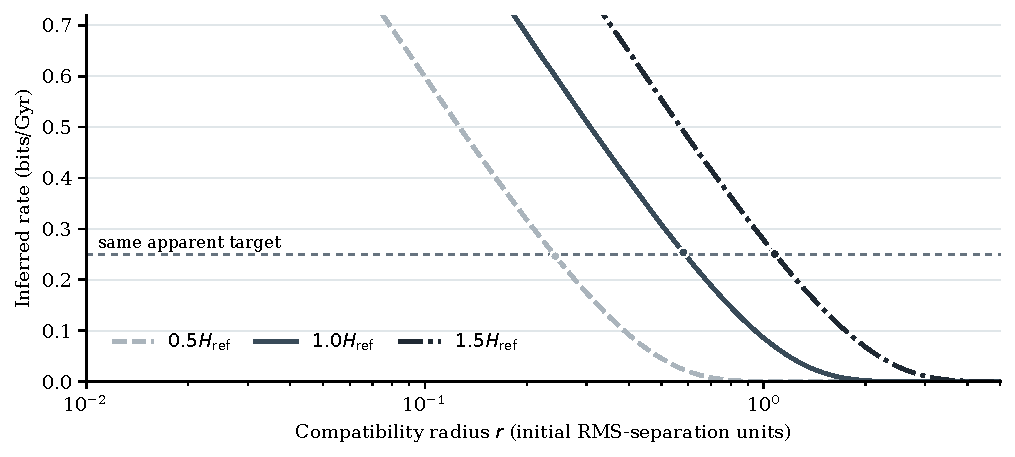
\includegraphics[width=0.91\linewidth]{radius_identifiability.pdf}
\caption{The inferred rate is a continuous function of the geometric
tolerance.  Each expansion history crosses the same apparent target (dots) at
a different radius, and none develops a stable one-decade plateau.  The
radius therefore selects the reported rate rather than revealing an invariant
one.}
\label{fig:radius-identifiability}
\end{figure}

Initial-resolution normalization collapsed exactly, and changing the slicing
from $20$ to $80$ steps altered cumulative distance by only
$1.49\times10^{-14}$.  The observed radius dependence is therefore the
mathematical behavior of the continuous-distance survival probability, not a
numerical artifact.  Geometric tolerance is useful once a physical resolution
is already known; it cannot by itself supply that resolution.

This conclusion points naturally to conservation laws.  Rather than declaring
histories compatible because they lie within an adjustable distance, one can
ask whether they satisfy the constraints that make them dynamically
admissible.

\begin{persuasions}
\item A percent-level error in an assumed expansion law can manufacture the
entire information rate the model seeks to explain.
\item Scanning the full radius curve is decisive: there is no stable plateau
hidden behind a fortunate choice of tolerance.
\item The desired rate needs a physically specified admissible set, not a
geometric radius chosen after seeing the result.
\item Conservation provides exactly that kind of specification.  It says which
transitions are allowed before their cardinality is counted.
\end{persuasions}

\section*{Noether symmetry defines admissible transitions}

Let $x$ be position and $p$ its conjugate momentum, so $(x,p)$ is one
canonical pair in phase space, the space of instantaneous mechanical states.
For a time-independent Hamiltonian $H(x,p)$, the function that assigns energy
and generates time evolution, time-translation symmetry implies conservation
of energy by Noether's theorem \citep{Noether1918,Arnold1989}.
In a bounded discretized phase space $\mathcal S_\epsilon$, the companion note
on energy-transition cardinality defines the conserving candidates by
\begin{equation}
\mathcal C_{\epsilon,\tau}(E_0)
=\{w\in\mathcal S_\epsilon:|H(w)-E_0|\le\tau\},
\qquad
\rho_{\epsilon,\tau}
=\frac{|\mathcal C_{\epsilon,\tau}|}{|\mathcal S_\epsilon|}.
\label{eq:noether-set}
\end{equation}
Here $\epsilon$ is the linear cell scale, $E_0$ is the conserved energy,
$\tau\geq0$ is an energy half-width, and $|\cdot|$ denotes the number of
discrete states; $w$ denotes one such discretized state.  Its survival
information is $C_{\epsilon,\tau}=-\log_2\rho_{\epsilon,\tau}$, shortened to
$C_\epsilon$ when admissibility is fixed by exact cell intersection.  The
conservation law acts as a dimensional filter: one
independent scalar equation reduces the dimension by one, so admissible states
concentrate on a codimension-one energy shell
\citep{LandersNoether2026}.

Here the tolerance is removed as a free parameter.  Let each grid point denote
a full phase-space cell of width $\epsilon$.  A cell is admissible precisely
when the range of $H$ over that cell intersects the exact energy $E_0$.  The
effective energy uncertainty is therefore determined by discretization
geometry.  For the unit harmonic oscillator,
\begin{equation}
H(x,p)=\frac{x^2+p^2}{2},
\qquad E_0=1,
\label{eq:harmonic-hamiltonian}
\end{equation}
the minimum and maximum of $H$ on every rectangular cell can be evaluated
exactly.  The calculation uses the bounded domain
$\mathcal S=[-2,2]\times[-2,2]$ and units in which mass and oscillator
frequency are one.

The count confirms the expected structure.  Refining $\epsilon$ from $0.2$ to
$0.0125$ raises the raw information from $2.6666$ to $6.8125$ bits.  At the
three finest resolutions, every halving adds approximately one bit.  In
general, for a smooth single-constraint shell in an $n$-dimensional domain,
\begin{equation}
|\mathcal S_\epsilon|\sim V\epsilon^{-n},
\qquad
|\mathcal C_\epsilon|\sim A_{\rm grid}\epsilon^{-(n-1)},
\qquad
C_\epsilon
=\log_2\frac1\epsilon-\log_2\frac{A_{\rm grid}}V+o(1).
\label{eq:codimension-scaling}
\end{equation}
Here $n$ is the phase-space dimension, $V$ is the coordinate volume of the
bounded domain, $A_{\rm grid}$ is the shell-content coefficient induced by the
chosen grid, $\sim$ denotes asymptotic equality as $\epsilon\to0$, and $o(1)$
is a term that vanishes in that limit.  The coefficient of
$\log_2(1/\epsilon)$ is not a nuisance discovered by the
simulation; it is the signature of one independent conservation constraint.

\begin{center}
\captionof{table}{Energy-shell cardinality for the harmonic oscillator.  The
raw count acquires one bit per spatial refinement; subtracting the universal
codimension term leaves a convergent grid-dependent finite part.}
\label{tab:energy-shell}
\small
\begin{tabular}{rrrr}
\toprule
$\epsilon$ & Conserving/total cells & $C_\epsilon$ (bits) &
$C_\epsilon-\log_2(1/\epsilon)$\\
\midrule
$0.2000$ & $63/400$ & $2.6666$ & $0.3446$\\
$0.1000$ & $120/1600$ & $3.7370$ & $0.4150$\\
$0.0500$ & $224/6400$ & $4.8365$ & $0.5146$\\
$0.0250$ & $448/25600$ & $5.8365$ & $0.5146$\\
$0.0125$ & $911/102400$ & $6.8125$ & $0.4906$\\
\bottomrule
\end{tabular}
\end{center}

\begin{persuasions}
\item Noether's theorem supplies more than a metaphor for compatibility.
Time symmetry selects an energy shell before any counting begins.
\item Grid cells that intersect the shell define ``almost conserving'' without
an adjustable energy tolerance: the uncertainty is fixed by the cell.
\item One bit per halving is the numerical image of codimension one.  The
growth has a geometric explanation rather than a fitted rate.
\item The finite remainder is the next candidate---but it must still pass the
invariance tests required of a physical quantity.
\end{persuasions}

\section*{From one transition to stationary-action histories}

Energy-shell cardinality concerns candidate states.  Accumulated history asks
which sequences of states remain dynamically admissible.  For the unit
harmonic-oscillator Lagrangian---the function whose time integral is the
action $S=\int L\,dt$---
\begin{equation}
L(x,\dot x)=\frac12\dot x^2-\frac12x^2,
\label{eq:lagrangian}
\end{equation}
where $\dot x=dx/dt$, stationarity ($\delta S=0$ under small path variations
with fixed endpoints) of the discretized action gives the central
Euler--Lagrange residual
\begin{equation}
R_m=x_{m+1}+(-2+\Delta t^2)x_m+x_{m-1}=0.
\label{eq:discrete-el}
\end{equation}
Here $m$ labels a time slice, $\Delta t$ is the constant interval between
slices, $x_m=x(m\Delta t)$, and $R_m$ measures failure of the discrete
equation of motion.  Given three position cells of width $\epsilon$, interval
arithmetic determines the exact range of $R_m$.  A candidate continuation is
admitted when that range contains zero.  The associated residual half-width,
\begin{equation}
\tau_R(\epsilon,\Delta t)
=\frac\epsilon2\left[2+|-2+\Delta t^2|\right],
\label{eq:residual-width}
\end{equation}
is derived from the cells and Eq.~\eqref{eq:discrete-el}; it is not adjusted to
the result.

Starting from cells containing $x(0)=1$ and
$x(\Delta t)=\cos\Delta t$ in the position domain $[-1.5,1.5]$, a dynamic
program propagates the fraction of next cells, proposed uniformly from that
domain, that satisfy every accumulated residual constraint.  At
$\Delta t=0.2$, raw
information per accepted update grows from $2.0919$ to $5.9069$ bits over the
tested refinement range.  Subtracting the same
$\log_2(1/\epsilon)$ term produces a stable finest-grid value near $-0.415$
bits per update.

Time refinement reveals a second continuum factor.  At fixed duration $2.4$
and $\epsilon=0.025$, halving $\Delta t$ approximately doubles the number of
constraints and therefore the accumulated information per unit time
(Table~\ref{tab:action-time}).  A continuum path is constrained at infinitely
many slices, so raw path cardinality requires a temporal measure just as state
cardinality requires a phase-space measure.

\begin{center}
\captionof{table}{Fixed-duration stationary-action histories.  Spatial
admissibility is physically defined, but raw information per unit time retains
the normalization of the temporal slicing.}
\label{tab:action-time}
\small
\begin{tabular}{rrrr}
\toprule
$\Delta t$ & Accepted updates & Total information (bits) & Bits/unit time\\
\midrule
$0.400$ & $5$ & $24.6457$ & $10.2690$\\
$0.200$ & $11$ & $54.0137$ & $22.5057$\\
$0.100$ & $23$ & $113.5199$ & $47.3000$\\
\bottomrule
\end{tabular}
\end{center}

This is significant progress in the definition of the problem.  The arbitrary
radius has disappeared; what remains is the familiar continuum question of
how a measure is normalized.  The spatial divergence exposes constraint
codimension.  The temporal divergence exposes the density of imposed slices.
Both can be separated from finite dynamical content, but only an invariant
construction can decide which finite content is physical.

\begin{persuasions}
\item Stationary action turns a one-step conservation shell into a filtration
of entire admissible paths.
\item The interval tolerance is calculated from the discretized equation of
motion.  There is no radius left to tune to a desired bit rate.
\item Spatial and temporal divergences are structurally informative: they
count constraint codimension and constraint density.
\item A continuum history theory therefore needs a measure on paths, not a
literal count of coordinate cells or time slices.
\end{persuasions}

\section*{Canonical invariance selects Liouville measure}

The convergent finite cell-count term is tempting, but convergence within one
grid is weaker than physical invariance.  The same harmonic shell was therefore
counted with equal-area rectangular cells of aspect ratios $0.5$, $1$, and $2$,
and after the canonical shear
\begin{equation}
Q=x,
\qquad P=p+x,
\qquad dx\wedge dp=dQ\wedge dP.
\label{eq:canonical-shear}
\end{equation}
Here $(Q,P)$ are new canonical coordinates and $\wedge$ is the antisymmetric
differential product defining oriented phase area; the last equality states
that the transformation preserves that area.  At the finest common cell area,
the codimension-subtracted finite terms were
$0.1773$, $0.4906$, $0.1773$, and $0.2225$ bits, respectively.  Their
$0.3134$-bit spread persists in the refinement limit.  Intersecting-cell count
measures an anisotropic grid perimeter; it is not a canonical scalar.

Hamiltonian mechanics supplies the appropriate replacement.  Liouville
measure
\begin{equation}
d\Gamma=dx\,dp
\label{eq:liouville-measure}
\end{equation}
is the phase-area element for one canonical pair; in $n$ pairs it is the
product $d\Gamma=\prod_{k=1}^n dx_k\,dp_k$.  It is preserved by Hamiltonian
flow and by canonical transformations
\citep{Liouville1838,Arnold1989}.  For a physical energy half-width $\tau_E$,
define the band density
\begin{equation}
g_{\tau_E}(E)
=\frac{1}{2\tau_E}
\int\mathbf1\{|H(x,p)-E|\le\tau_E\}\,d\Gamma.
\label{eq:band-density}
\end{equation}
Here $\mathbf1\{\cdot\}$ is one when its condition holds and zero otherwise,
and $\tau_E>0$ is a fixed physical energy half-width.  Thus $g_{\tau_E}$ is
phase volume per unit energy.  As $\tau_E\to0$, this approaches the
microcanonical density of states
\begin{equation}
g(E)=\int\delta(H-E)\,d\Gamma,
\label{eq:density-of-states}
\end{equation}
where $\delta$ is the Dirac delta distribution, which restricts the integral
to the energy surface.  Unlike cell incidence, Eq.~\eqref{eq:band-density}
weights every cell by its phase volume.

The invariance test used $\tau_E=0.05$.  For the harmonic oscillator, the exact
band density is $2\pi=6.283185$.  Across all aspect ratios and the canonical
shear, numerical estimates ranged from $6.283000$ to $6.290000$: a maximum
relative error of $0.108\%$ and cross-scheme spread of $0.111\%$.  A second,
anharmonic Hamiltonian,
\begin{equation}
H_{\rm anh}(x,p)=\frac{p^2}{2}+\frac{x^2}{2}+\frac{x^4}{8},
\label{eq:anharmonic}
\end{equation}
has reference band density $5.061875$, obtained by high-accuracy quadrature of
the enclosed phase volume.  The same schemes returned $5.058000$ to
$5.071000$, with maximum error $0.180\%$ and cross-scheme spread $0.257\%$.

\begin{center}
\captionof{table}{Canonical and grid invariance at the finest tested
quadrature.  Raw cell finite parts vary materially; Liouville band densities
agree with the invariant reference values for two Hamiltonians.}
\label{tab:invariance}
\small
\begin{tabular}{lrrr}
\toprule
Scheme & Cell finite part & Harmonic $g_{\tau_E}$ & Anharmonic $g_{\tau_E}$\\
\midrule
Aspect $0.5$ & $0.1773$ & $6.284000$ & $5.065000$\\
Aspect $1$ & $0.4906$ & $6.290000$ & $5.071000$\\
Aspect $2$ & $0.1773$ & $6.284000$ & $5.058000$\\
Canonical shear & $0.2225$ & $6.283000$ & $5.058000$\\
Reference invariant & --- & $6.283185$ & $5.061875$\\
\bottomrule
\end{tabular}
\end{center}

The split is unambiguous.  Raw cardinality knows about the coordinate lattice.
Liouville density knows about the Hamiltonian system.  The first is a useful
regularization diagnostic; the second is an invariant candidate for physical
history measure.

\begin{persuasions}
\item A convergent number is not automatically a physical number.  It must
survive coordinate transformations that leave the dynamics unchanged.
\item Grid-cell incidence fails that test because different cell shapes cover
the same shell differently.
\item Liouville measure passes across grids, canonical coordinates, and both
tested Hamiltonians.
\end{persuasions}

\begin{figure}[ht]
\centering
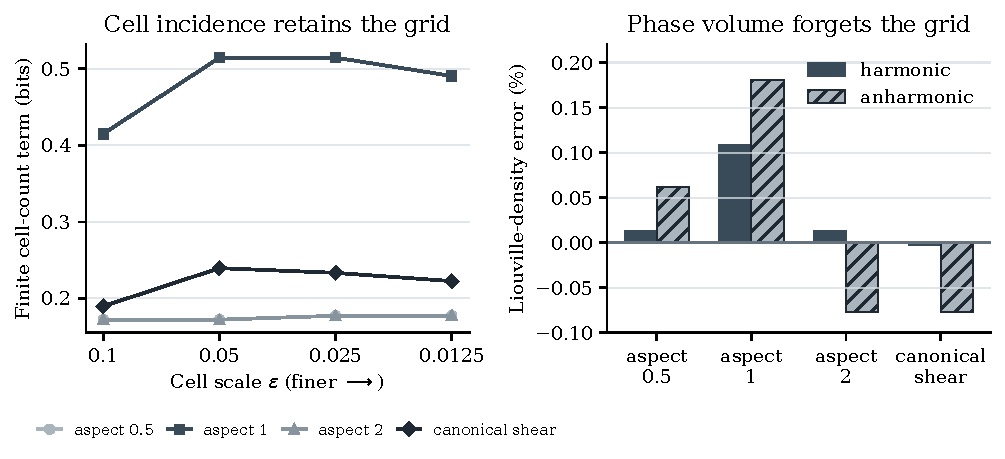
\includegraphics[width=0.98\linewidth]{measure_invariance.pdf}
\caption{Two refinement tests separate regularization from physics.  Left:
after subtracting the universal codimension term, cell-incidence counts
approach different finite values for different grids and canonical
coordinates.  Right: Liouville band density at the finest quadrature remains
within $0.18\%$ of the invariant reference value for every scheme and both
Hamiltonians.}
\label{fig:measure-invariance}
\end{figure}

\section*{The revised cosmological object}

The result suggests a precise refinement of Eq.~\eqref{eq:survival}.  Let
$\mathcal P_n$ be the set of candidate continuations at causal slice $n$, let
$\mathcal A_n\subseteq\mathcal P_n$ be the subset satisfying the dynamical
constraints given the shared past, and let $\mu$ be the invariant measure
appropriate to the system.  Write $\mathcal A_{<n}$ for all admissibility
conditions imposed on slices before $n$.  The conditional survival information
added at slice $n$ is
\begin{equation}
\Delta C_\mu(n)
=-\log_2
\frac{\mu(\mathcal A_n\mid\mathcal A_{<n})}
     {\mu(\mathcal P_n\mid\mathcal A_{<n})}.
\label{eq:conditional-measure}
\end{equation}
The notation $\mu(B\mid A)$ means the measure assigned to $B$ after
conditioning on $A$; the ratio is the surviving fraction of candidate
measure.  For classical Hamiltonian systems, the present tests select
Liouville measure
over coordinate-cell count.  For fields or gravity, the analogue must respect
the constrained symplectic structure (the geometry defined by canonical
coordinates and their conserved phase volume) and gauge redundancy (different
mathematical descriptions of the same physical state).  For relativistic
histories it must additionally respect causal order and proper-time slicing.

Through slice $N$, define the accumulated information by
\begin{equation}
C_\mu(N)=\sum_{n=1}^{N}\Delta C_\mu(n),
\qquad C_\mu(0)=0,
\label{eq:accumulated-measure}
\end{equation}
and let $C_\mu(\tau)$ denote a continuum interpolation when the refinement
limit exists.  Thus $\Delta C_\mu$ is the new conditional information at one
slice, while $C_\mu$ is the accumulated history quantity.

Equation~\eqref{eq:conditional-measure} is dimensionless when numerator and
denominator are positive-measure sets of the same phase dimension.  Exact
constraint surfaces instead require an induced measure, a physical band, or a
relative density such as $g(E)/g_*(E)$, where $g_*$ is an independently
specified reference density with the same units as $g$.  An absolute number of
phase-space states introduces an action cell; quantum mechanics naturally
supplies a scale of order Planck's constant $h$ per canonical pair, whereas a
purely classical theory does not.
The normalization is therefore a physical question, not a parameter to be
chosen for cosmological agreement.

The cosmological bridge can now be stated with greater discipline:
\begin{equation}
H_{\rm rel}(\tau)
=\frac{\ln2}{3}\,
\frac{d C_\mu}{d\tau},
\label{eq:revised-bridge}
\end{equation}
where $\tau$ is an invariant time parameter, such as proper time, along the
relevant congruence (a family of neighboring observer worldlines) and $C_\mu$
is built from conditional invariant measure.  The equation remains a
constitutive hypothesis, but its information variable is no longer an
arbitrary neighborhood count.  Its open ingredients are sharply located:
the gravitational history measure, the treatment of constraints and gauge,
and the continuum normalization of successive causal slices.

The earlier Hubble-scale result gives a quantitative target for this object.
At the present epoch, Eq.~\eqref{eq:revised-bridge} asks for an invariant
conditional rate of order $0.25$--$0.31\,\mathrm{bits/Gyr}$, depending on
whether one isolates the late-time constant component or uses the full
$H_0$.  That number should emerge only after the measure and normalization are
fixed.  The new results make clear what must be derived before it is compared
with cosmological data.

\begin{persuasions}
\item The compatible-history idea survives in a stronger form: probability is
replaced by conditional invariant measure.
\item Noether constraints define admissibility; Liouville geometry defines how
admissible alternatives are weighted.
\item A quantum action cell is a natural candidate for making phase volume
dimensionless, while a covariant path measure must resolve the temporal
continuum.
\item The Hubble-scale bit rate is now a target for an invariant construction,
not a value used to choose its tolerance or cutoff.
\end{persuasions}

\section*{Constructive outlook}

The accumulated-history program began with the observation that a longer past
can distinguish histories that once appeared equivalent.  Its simplest
cosmological realization found the correct present Hubble scale, then learned
from the expansion history that the relevant information rate must be
dynamical.  The experiments reported here advance the next layer.

First, conditional survival separates genuinely unresolved distinctions from
predictable expansion and chaos.  Second, the absence of a stable geometric
radius shows why compatibility must be supplied by physics.  Third, Noether
symmetry and stationary action supply that admissibility without fitting a
tolerance.  Fourth, continuum refinement separates universal constraint terms
from finite content.  Finally, canonical tests select Liouville measure and
exclude raw cell incidence as the physical finite quantity.

The next calculation is consequently well defined.  Construct the constrained
symplectic measure for a finite gravitational or cosmological system, define
the conditional measure added by successive causal slices, and test whether a
renormalized rate converges under simultaneous phase-space and temporal
refinement.  Only then should the rate be compared with
$H=(\ln2/3)\dot C_\mu$ and the held-out DESI expansion history.

The central promise has become more concrete.  Accumulated history need not be
counted by arbitrary coordinates; symmetry can define the admissible roads,
and invariant measure can say how much room those roads occupy.  The remaining
problem is no longer what should be counted.  It is how the invariant measure
of newly admissible history flows in a relativistic universe.

\begin{persuasions}
\item The program has moved from analogy to a tested measurement hierarchy:
conditional prediction, physical admissibility, continuum analysis, and
canonical invariance.
\item Noether's theorem identifies the roads; Liouville measure replaces the
coordinate-dependent count of paving stones.
\item The surviving question is precise: does invariant compatible-history
measure flow at the Hubble rate?  The near equality $H_0\simeq1/t_0$ fixes the
motivating present target.
\end{persuasions}

\bibliographystyle{unsrtnat}
\bibliography{../../references/complexity_cosmology}

\end{document}
